%-------------------------------------------------------------------------------
%                                PREAMBLE
%-------------------------------------------------------------------------------
\documentclass[usenames,dvipsnames,svgnames,10pt,aspectratio=169]{beamer}
%
\usefonttheme{professionalfonts}
% This theme uses TIKZ: compile twice with PDFLaTeX or LuaLaTeX.
%
%  Options:
%  - [clean]:    clean slides, i.e. logos and footbar are removed
%  - [kth]:      footbar style inspierd to the official KTH template
%  - [nicewave]: a different style of wave is used (not approved by FLOW)
%
\usetheme[clean]{flow}

\usepackage{tikz}
\usepackage{pgfplots}
\usepgfplotslibrary{polar}

\usepackage{hyperref,graphicx,lmodern}
\usepackage[utf8]{inputenc}
\usepackage{media9}
\usepackage{xcolor}
\usepackage{stmaryrd}
\usepackage{nicefrac}
\usepackage{multimedia}
\usepackage{multicol}
\usepackage{upgreek}
\usepackage[]{bm}
\usepackage[]{url}
\usepackage[]{animate}
\usepackage{amsmath}

\graphicspath{{imgs/}}
\setbeamertemplate{blocks}[rounded][shadow=true]


\usepackage[]{listings}

\definecolor{codegreen}{rgb}{0,0.6,0}
\definecolor{codegray}{rgb}{0.5,0.5,0.5}
\definecolor{codepurple}{rgb}{0.58,0,0.82}
\definecolor{backcolour}{rgb}{1.0, 1.0, 1.0}

\lstdefinestyle{mystyle}{
  backgroundcolor=\color{backcolour},
  commentstyle=\color{codegreen},
  keywordstyle=\color{magenta},
  numberstyle=\tiny\color{codegray},
  stringstyle=\color{codepurple},
  basicstyle=\ttfamily\footnotesize,
  breakatwhitespace=false,
  breaklines=true,
  captionpos=b,
  keepspaces=true,
  numbers=left,
  numbersep=5pt,
  showspaces=false,
  showstringspaces=false,
  showtabs=false,
  tabsize=2
}

\lstset{style=mystyle}


%-------------------------------------------------------------------------------
%                                TITLE PAGE
%-------------------------------------------------------------------------------
\title[Nonlinear physics] % Short title used in footline
{
	Introduction au calcul scientifique
}

\author[J.-Ch.~Loiseau] % Presenting author in short form used in footline
{
	\underline{Jean-Christophe Loiseau}
}
% - Give the names in the same order as the appear in the paper.
% - Underline the presenting author.

\institute[unused]
{
	\url{jean-christophe.loiseau@ensam.eu} \\
	Laboratoire DynFluid \\
	Arts et M\'etiers, France.
}
% Keep it simple, no one is interested in your street address.

% University logo(s)
\logot{
\includegraphics[width=.128\paperwidth]{DynFluid_logo}}  % Top logo
\logob{
\includegraphics[width=0.128\paperwidth]{ENSAM_logo}} % Bottom logo
% \logoc[{\includegraphics[width=.128\paperwidth]{limsi}}]{\includegraphics[width=.128\paperwidth]{limsi}} % Corner logo
%
% Cover image: \cvrimg{x position}{y position}{cover image}
\cvrimg{.77}{.8}{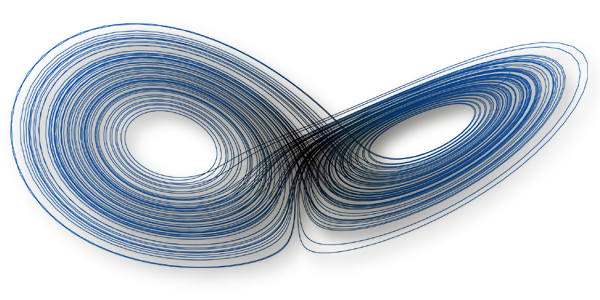
\includegraphics[width=.4\paperwidth]{cover.png}}

\date[unused]{Physique non-lin\'eaire -- 2019-2020}

\begin{document}

\titleframe	% Print the title as the first slide

%-------------------------------------------------------------------------------
%                           PRESENTATION SLIDES
%-------------------------------------------------------------------------------

\begin{frame}[t, c]{Simulation numérique}{}
	\begin{minipage}{.68\textwidth}
    Avec l'accroissement de nos capacités de calcul, la \alert{\textbf{simulation numérique}} est devenue aujourd'hui l'un des outils les plus utilisés en ingénierie.

    \bigskip

    Etre capable de simuler efficacement, précisément et rapidement les \alert{\textbf{équations différentielles}} décrivant l'évolution de systèmes potentiellement très complexes est donc d'une importance capitale.
	\end{minipage}%
	\hfill
	\begin{minipage}{.28\textwidth}
    \centering
    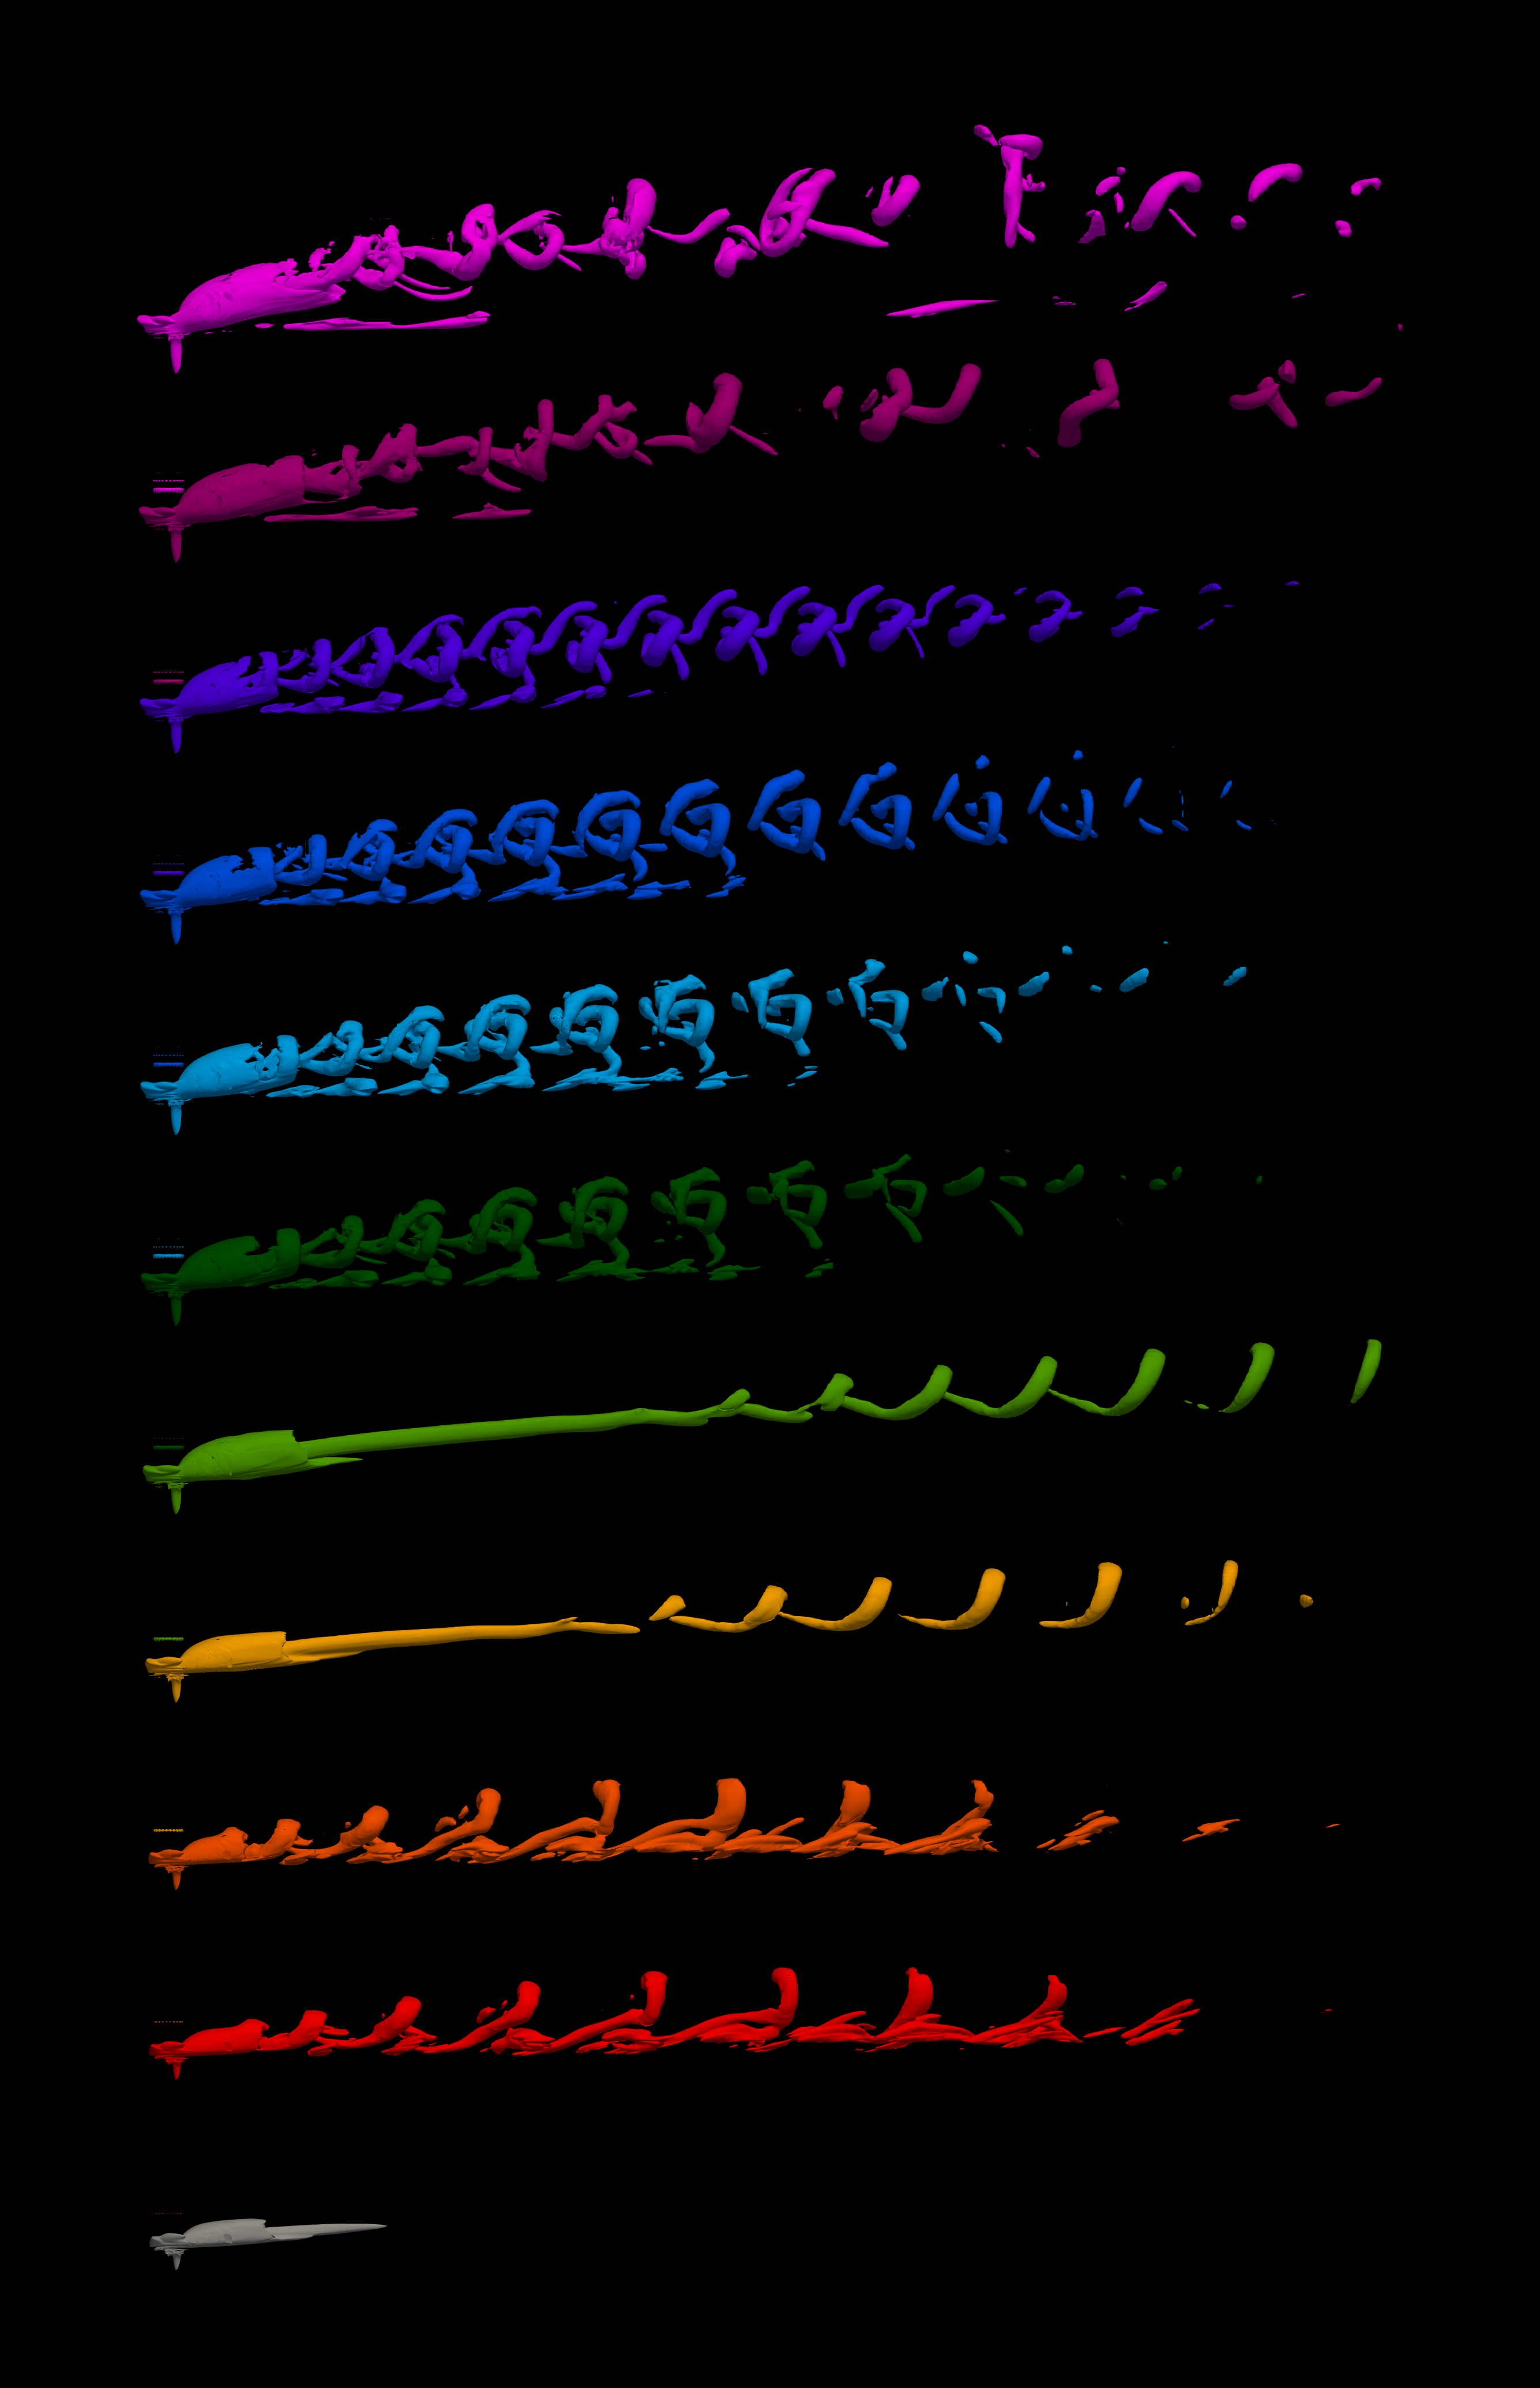
\includegraphics[width=\textwidth]{jet_in_xflow}
	\end{minipage}

	\vspace{1cm}
\end{frame}

\begin{frame}[t, c]{Simulation numérique}{}
  \centering
  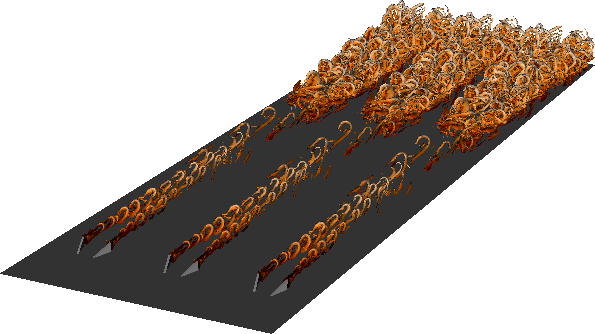
\includegraphics[width=.8\textwidth]{instability_and_transition}
\end{frame}

\begin{frame}[t, c]{Simulation numérique}{}
  Il existe deux grandes familles d'équations différentielles :
  %
  \begin{itemize}
  \item Les \alert{\textbf{équations différentielles ordinaires}} permettent de modéliser des systèmes dont l'évolution ne dépend que du temps.
    Elles sont en générales de la forme
    %
    \[
    \dfrac{d\bm{x}}{dt} = \bm{f}(t, \bm{x}, \bm{u})
    \]
    %
    avec $\bm{x} \in \mathbb{R}^n$ le vecteur d'état et $\bm{u}$ une action externe (e.g.\ loi de contrôle).

    \medskip

  \item Les \alert{\textbf{équations aux dérivées partielles}} permettent quant à elles de simuler des systèmes dont l'évolution dépend du temps et de l'espace.
    L'exemple le plus connu sont les équations de Navier-Stokes
    %
    \[
    \begin{aligned}
      \dfrac{\partial \bm{u}}{\partial t} + \nabla \cdot \left( \bm{u} \otimes \bm{u} \right) & = - \nabla p + \dfrac{1}{Re} \nabla^2 \bm{u} \\
      \nabla \cdot \bm{u} & = 0
    \end{aligned}
    \]
    %
    où le champ de vitesse $\bm{u}$ dépend du temps et de l'espace.
  \end{itemize}

  \vspace{1cm}
\end{frame}

\begin{frame}[t, c]{Equations différentielles ordinaires}{Linear-time invariant dynamical systems}
  \begin{minipage}{.68\textwidth}
    Intéressons-nous tout d'abord à des systèmes linéaires du type
    %
    \[
    \begin{aligned}
      \dot{\bm{x}} & = \bm{Ax} + \bm{Bu} \\
      \bm{y} & = \bm{Cx} + \bm{Du}.
    \end{aligned}
    \]
    %
    Ici, $\bm{x} \in \mathbb{R}^n$ est le vecteur d'état, $\bm{u} \in \mathbb{R}^p$ les inputs et $\bm{y} \in \mathbb{R}^q$ les mesures faites au cours du temps.
  \end{minipage}%
  \hfill
  \begin{minipage}{.28\textwidth}
  \end{minipage}
\end{frame}

\begin{frame}[t, c]{Equations différentielles ordinaires}{Linear-time invariant dynamical systems}
  \begin{minipage}{.68\textwidth}
    Si $\bm{u}(t)$ est connu à l'avance, alors la solution du système s'écrit
    %
    \[
    \bm{x}(t) = e^{t \bm{A}} \bm{x}_0 + \int_0^t e^{(t-\tau) \bm{A}} \bm{Bu}(\tau) \ \mathrm{d}\tau.
    \]
    %
    Le premier terme correspond à la \alert{\textbf{réponse naturelle}} (ou homogène) tandis que le second décrit la \alert{\textbf{réponse forcée}} du système.
  \end{minipage}%
  \hfill
  \begin{minipage}{.28\textwidth}

  \end{minipage}
\end{frame}

\begin{frame}[t, c]{Equations différentielles ordinaires}{Linear-time invariant dynamical systems}
  
\end{frame}

\begin{frame}[t, c]{Equations différentielles ordinaires}{Linear-time invariant dynamical systems}
  \begin{minipage}{.68\textwidth}
    L'exponentielle d'une matrice est définie comme
    %
    \[
    e^{\bm{A}} = \bm{V} e^{\boldsymbol{\Lambda}} \bm{V}^{-1}
    \]
    %
    où $\bm{V}$ est la matrice des vecteurs propres et $\boldsymbol{\Lambda}$ est une matrice diagonale dont les entrées sont les valeurs propres.

    \bigskip

    Pour des problèmes de grande taille, calculer ces valeurs propres et vecteurs propres peut néanmoins s'avérer extrêmement compliqué.
  \end{minipage}%
  \hfill
  \begin{minipage}{.28\textwidth}
  \end{minipage}
\end{frame}

\begin{frame}[t, c]{Equations différentielles ordinaires}{Linear-time invariant dynamical systems}
  \begin{minipage}{.68\textwidth}
    Comment faire alors pour simuler \( \dot{\bm{x}} = \bm{Ax} + \bm{Bu} \) ?
    Pour cela, on va avoir besoin de \alert{\textbf{discrétiser}} l'équation, i.e. considérer la solution à des intervalles de temps réguliers $t_k = k \Delta t$ avec $\Delta t$ le \alert{\textbf{pas de temps}}.
  \end{minipage}%
  \hfill
  \begin{minipage}{.28\textwidth}
    
  \end{minipage}
\end{frame}

\begin{frame}[t, c]{Equations différentielles ordinaires}{Linear-time invariant dynamical systems}
  \begin{minipage}{.68\textwidth}
    En absence de forçage externe, la solution au temps $t_{k+1} = (k+1)\Delta t$ est donnée par
    %
    \[
    \bm{x}_{k+1} = e^{\Delta t \bm{A}} \bm{x}_k.
    \]
    %
    Si $\Delta t$ est suffisament petit, on peut alors approximer l'exponentielle par son développement de Taylor
    %
    \[
    e^{\Delta t \bm{A}} = \bm{I} + \Delta t \bm{A} + \mathcal{O}(\Delta t^2)
    \]
    %
    ce qui nous donne alors
    %
    \[
    \bm{x}_{k+1} = \bm{x}_k + \Delta t \bm{Ax}_k + \mathcal{O}(\Delta t^2).
    \]
  \end{minipage}%
  \hfill
  \begin{minipage}{.28\textwidth}
  \end{minipage}
\end{frame}

\begin{frame}[t, c]{Equations différentielles ordinaires}{Linear-time invariant dynamical systems}
  \begin{minipage}{.68\textwidth}
    L'approximation $\bm{x}_{k+1} = \bm{x}_k + \Delta t \bm{Ax}_k$ est ce qu'on appelle le \alert{\textbf{schéma d'Euler explicite du premier ordre}}.
    Il correspond à l'approximation suivante du système
    %
    \[
    \dot{\bm{x}} = \bm{Ax} \to \dfrac{\bm{x}_{k+1} - \bm{x}_k}{\Delta t} = \bm{Ax}_k.
    \]
    %
    Il en existe de nombreuses variantes plus ou moins précises et plus ou moins couteuses en temps de calcul.
  \end{minipage}%
  \hfill
  \begin{minipage}{.28\textwidth}
    \centering
    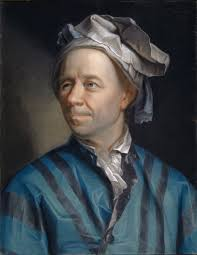
\includegraphics[width=\textwidth]{euler}
  \end{minipage}
\end{frame}

\begin{frame}[t, c]{Equations différentielles ordinaires}{Linear-time invariant dynamical systems}
  \alert{\textbf{Schéma d'Euler implicite du premier ordre}} : La solution au temps $t_k$ peut également s'écrire
    %
    \[
    e^{-\Delta t \bm{A}} \bm{x}_{k+1} = \bm{x}_k.
    \]
    %
    De la même façon, un développement limité au premier ordre donne
    %
    \[
    \begin{aligned}
      & \left( \bm{I} - \Delta t \bm{A} \right) \bm{x}_{k+1} = \bm{x}_k \\
      & \bm{x}_{k+1} = \left( \bm{I} - \Delta t \bm{A} \right)^{-1} \bm{x}_k
    \end{aligned}
    \]
    %
    Il correspond à l'approximation suivante du système
    %
    \[
    \dot{\bm{x}} = \bm{Ax} \to \dfrac{\bm{x}_{k+1} - \bm{x}_k}{\Delta t} = \bm{Ax}_{k+1}.
    \]
\end{frame}

\begin{frame}[t, c]{Equations différentielles ordinaires}{Linear-time invariant dynamical systems}
  \alert{\textbf{Schéma de Crank-Nicholson du deuxième ordre}} : La solution au temps $t_k$ peut également s'écrire
  %
  \[
  e^{-\nicefrac{\Delta t}{2} \bm{A}} \bm{x}_{k+1} = e^{\nicefrac{\Delta t}{2} \bm{A}} \bm{x}_{k}
  \]
  %
  Un développement limité de l'exponentielle à droite et à gauche du signe égal donne
  %
  \[
  \begin{aligned}
    & \left( \bm{I} - \dfrac{\Delta t}{2} \bm{A} \right) \bm{x}_{k+1} = \left( \bm{I} + \dfrac{\Delta t}{2} \bm{A} \right) \bm{x}_k \\
    & \bm{x}_{k+1} = \left( \bm{I} - \dfrac{\Delta t}{2} \bm{A} \right)^{-1} \left( \bm{I} + \dfrac{\Delta t}{2} \bm{A} \right) \bm{x}_k.
  \end{aligned}
  \]
  %
  Il correspond à l'approximation suivante du système
  %
  \[
  \dot{\bm{x}} = \bm{Ax} \to \dfrac{\bm{x}_{k+1} - \bm{x}_k}{\Delta t} = \dfrac{1}{2} \left( \bm{Ax}_{k+1} + \bm{Ax}_k \right).
  \]
\end{frame}

\begin{frame}[t, c]{Equations différentielles ordinaires}{Linear-time invariant dynamical systems}
  
\end{frame}

\begin{frame}[t, c]{Equations différentielles ordinaires}{Linear-time invariant dynamical systems}
  \centering
  \begin{tabular}{c|ccccc}
    Méthode & Implémentation & Coût de calcul & Robustesse & Choix de $\Delta t$ \\
    \hline
    \hline \\
    Explicite & {\color{green}Facile} & {\color{green} Peu cher} & {\color{red} Moyenne} & {\color{orange} Petit $\Delta t$}
    \\
    \\
    Implicite & {\color{orange} Plus compliqué} & {\color{orange} Plus cher} & {\color{green} Excellente} & {\color{green} Grand $\Delta t$}
  \end{tabular}
\end{frame}

\begin{frame}[t, c]{Equations différentielles ordinaires}{Systèmes non-linéaires}
  \begin{minipage}{.68\textwidth}
    La plupart des systèmes d'intérêt en pratique sont non-linéaires
    %
    \[
    \dot{\bm{x}} = \bm{f}(\bm{x})
    \]
    %
    avec $\bm{f} : \mathbb{R}^n \to \mathbb{R}^n$ une fonction non-linéaire qui ne respecte donc pas le principe de superposition, i.e.
    %
    \[
    \bm{f}(\alpha \bm{x}) \neq \alpha \bm{f}(\bm{x}) \quad \text{et} \quad \bm{f}(\bm{x} + \bm{y}) \neq \bm{f}(\bm{x}) + \bm{f}(\bm{y}).
    \]
    %
    Leur simulation repose néanmoins sur les mêmes principes.
  \end{minipage}%
  \hfill
  \begin{minipage}{.28\textwidth}
  \end{minipage}
\end{frame}

\begin{frame}[t, c]{Equations différentielles ordinaires}{Systèmes non-linéaires}
  \begin{minipage}{.68\textwidth}
    \begin{itemize}
    \item \alert{\textbf{Schéma d'Euler explicite du premier ordre}}
      %
      \[
      \bm{x}_{k+1} = \bm{x}_k + \Delta t \bm{f}(\bm{x}_k)
      \]

    \item \alert{\textbf{Schéma d'Euler implicite du premier ordre}}
      %
      \[
      \bm{x}_{k+1} - \Delta t \bm{f}(\bm{x}_{k+1}) = \bm{x}_k
      \]

    \item \alert{\textbf{Schéma de Crank-Nicholson du deuxième ordre}}
      %
      \[
      \bm{x}_{k+1} - \dfrac{\Delta t}{2} \bm{f}(\bm{x}_{k+1}) = \bm{x}_k + \dfrac{\Delta t}{2} \bm{f}(\bm{x}_k)
      \]
    \end{itemize}
  \end{minipage}%
  \hfill
  \begin{minipage}{.28\textwidth}
  \end{minipage}
\end{frame}

\begin{frame}[t, c, fragile]{Equations différentielles ordinaires}{Python}
  \begin{minipage}{.68\textwidth}
    En python, la simulation d'équations différentielles ordinaires se fait à l'aide de la fonction \verb+solve_ivp+ du package \verb+scipy.integrate+ donnant accès à de nombreuses méthodes d'intégration différentes.
  \end{minipage}%
  \hfill
  \begin{minipage}{.28\textwidth}
    \centering
    
\includegraphics[width=\textwidth]{scipy_logo}
  \end{minipage}
\end{frame}

\begin{frame}[t, c, fragile]{Equations différentielles ordinaires}{Python}
  \begin{minipage}{.68\textwidth}
    \begin{lstlisting}[language=Python]
      from scipy.integrate import solve_ivp

      # --> dx/dt = a x.
      def dynsys(t, x, a):
          return a*x

      # --> Parametres pour l'integration.
      tspan = (0.0, 10.0)
      teval = np.linspace(tspan[0], tspan[1], 1024)
      a = -0.1
      x0 = 1.0

      # --> Simulation.
      sol = solve_ivp(
          lambda t, x: dynsys(t, x, a),
          tspan,
          x0,
          teval=teval
          )
    \end{lstlisting}
  \end{minipage}%
  \hfill
  \begin{minipage}{.28\textwidth}
    \centering
    
\includegraphics[width=\textwidth]{scipy_logo}
  \end{minipage}
\end{frame}

\begin{frame}[t, c]{Equations différentielles ordinaires}{Exemple : le système de Lorenz}
  \begin{minipage}{.68\textwidth}
    Le système de Lorenz est un modèle très simplifié du phénomène de convection atmosphérique.
    Il est donné par
    %
    \[
    \begin{aligned}
      \dot{x} & = \sigma ( y - x ) \\
      \dot{y} & = x ( \rho - z) - y \\
      \dot{z} & = xy - \beta z.
    \end{aligned}
    \]
    %
    C'est l'un des systèmes historiquement les plus importants en théorie des systèmes dynamiques et notamment en théorie du chaos.
  \end{minipage}%
  \hfill
  \begin{minipage}{.28\textwidth}
    \centering
    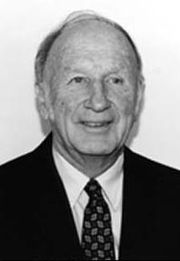
\includegraphics[width=\textwidth]{portrait_lorenz}
  \end{minipage}
\end{frame}

\begin{frame}[t, c, fragile]{Equations différentielles ordinaires}{Exemple : le système de Lorenz}
  \begin{minipage}{.48\textwidth}
    \begin{lstlisting}[language=Python]
      def dynsys(t, u, p):
          # Unpack parameters.
          sigma, rho, beta = p

          # Unpack variables.
          x, y, z = u

          # Lorenz system
          dx = sigma * ( y - x)
          dy = x * (rho - z) - y
          dz = x * y - beta *z

          return dx, dy, dz
    \end{lstlisting}
  \end{minipage}%
  \hfill
  \begin{minipage}{.48\textwidth}
    \begin{lstlisting}[language=Python]
      # Parametres du systeme.
      sigma, rho, beta = 10, 28, 8/3
      p = [sigma, rho, beta]

      # Parametres pour l'integration.
      tspan = (0.0, 20.0)
      u0 = np.array([1.0, 0.0, 0.0])

      # Simulation.
      sol = solve_ivp(
      lambda t, u : dynsys(t, u, p),
      tspan,
      x0)

    \end{lstlisting}
  \end{minipage}
\end{frame}

\begin{frame}[t, c]{Equations différentielles ordinaires}{Exemple : le système de Lorenz}
  \centering
  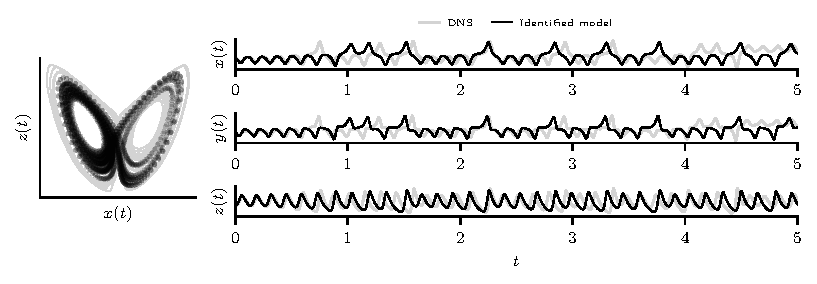
\includegraphics[width=\textwidth]{attractor_comparison}
\end{frame}

\begin{frame}[t, c]{Equations différentielles ordinaires}{Exemple : le système de Lorenz}
  \begin{minipage}{.68\textwidth}

    Le système de Lorenz présente la propriété de \alert{\textbf{sensibilité aux conditions initiales}} rendant toute prédiction précise inutile au delà d'une certaine échelle de temps.

    \bigskip

    \begin{center}
      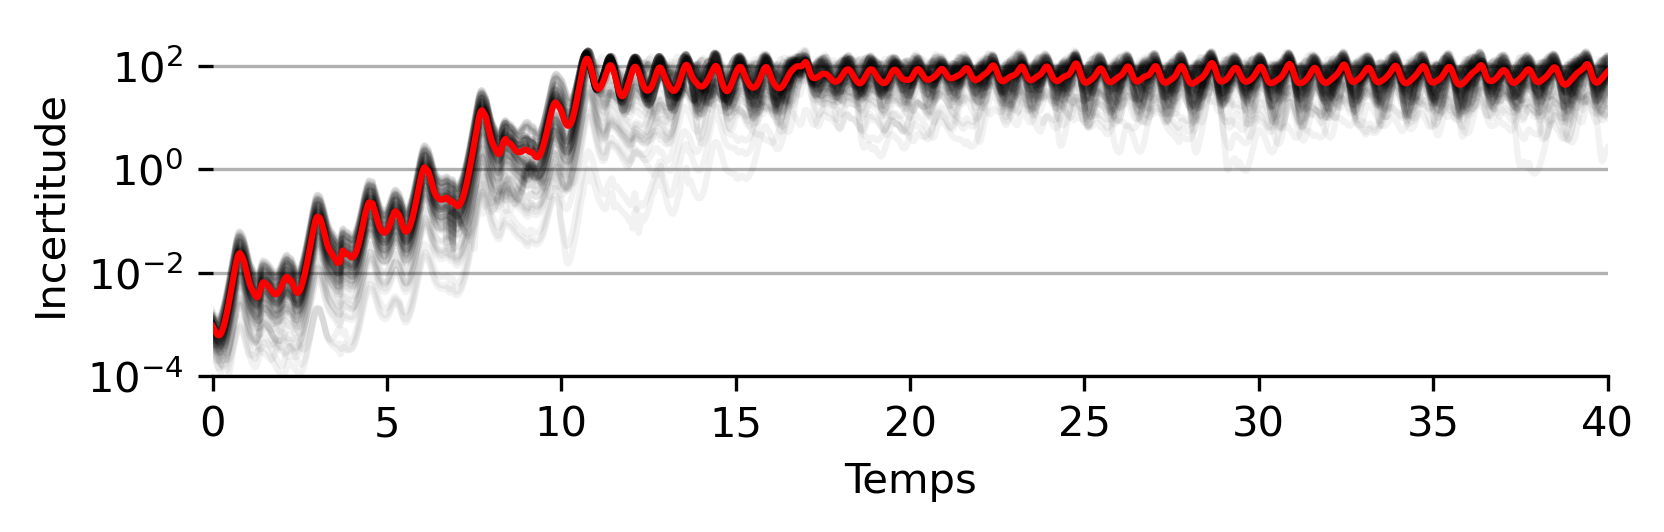
\includegraphics[width=\textwidth]{lorenz_forecast_error}
    \end{center}
  \end{minipage}%
  \hfill
  \begin{minipage}{.28\textwidth}
    \centering
    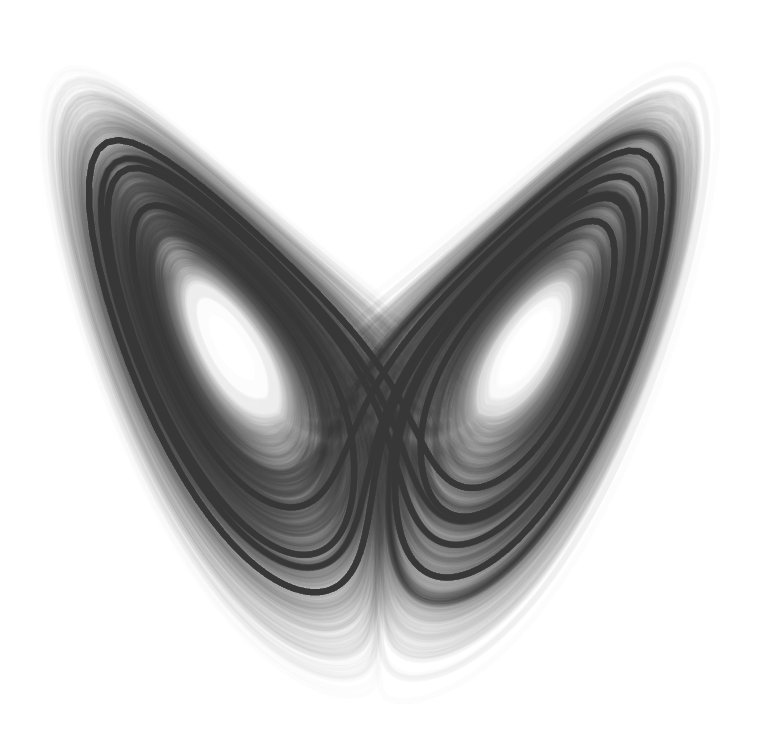
\includegraphics[width=\textwidth]{lorenz_attractor}
  \end{minipage}
\end{frame}

\begin{frame}[t, c]{Equations différentielles ordinaires}{Exemple : le modèle SIR}
  \begin{minipage}{.68\textwidth}
    Le modèle SIR est un modèle utilisé en épidémiologie pour modéliser l'évolution d'une épidémie.
    Il est donné par
    %
    \[
    \begin{aligned}
      \dfrac{dS}{dt} & = - \beta SI \\
      \dfrac{dI}{dt} & = \beta SI - \gamma I \\
      \dfrac{dR}{dt} & = \gamma I
    \end{aligned}
    \]
    %
    où $S$, $I$ et $R$ représentent respectivement la fraction de la population saine, actuellement infectée et s'étant remise de l'infection.
    Les paramètres $\beta$ et $\gamma$ caractérisent certaines propriétés du virus.
  \end{minipage}%
  \hfill
  \begin{minipage}{.28\textwidth}
    \centering
    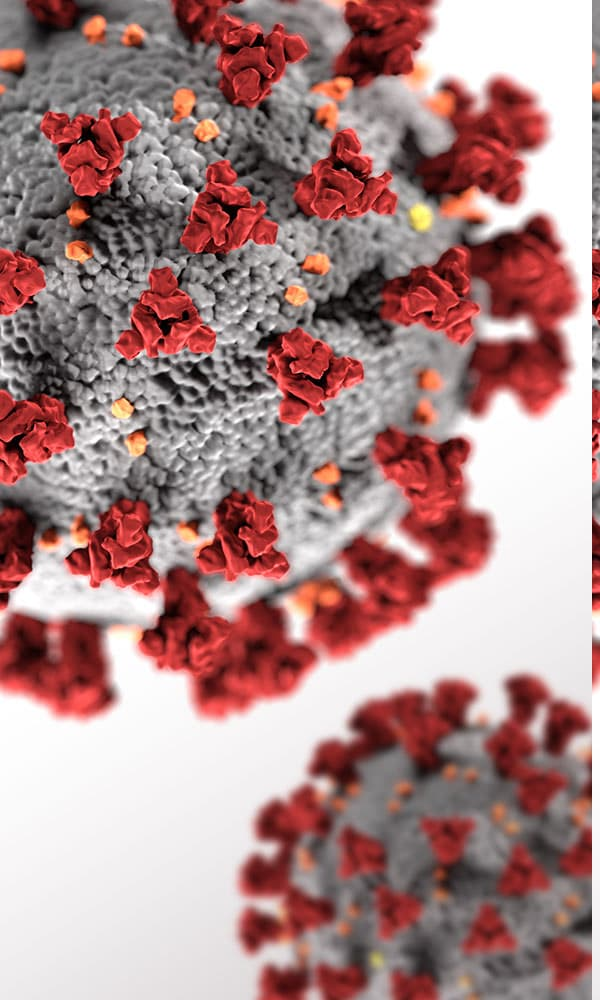
\includegraphics[width=.8\textwidth]{virus}
  \end{minipage}
\end{frame}

\begin{frame}[t, c, fragile]{Equations différentielles ordinaires}{Exemple : le modèle SIR}
  \begin{minipage}{.48\textwidth}
    \begin{lstlisting}[language=Python]
      def sir(t, u, p):
          # Unpack parameters.
          beta, gamma = p

          # Unpack variables.
          s, i, r = u

          # Equations.
          ds = - beta * s * i
          di = beta * s * i - gamma * i
          dr = gamma *i
          
          return ds, di, dr
    \end{lstlisting}
  \end{minipage}%
  \hfill
  \begin{minipage}{.48\textwidth}
    \begin{lstlisting}[language=Python]
      # Parametres de l'epidemie.
      beta, gamma = 1.0, 1.0
      p = [beta, gamma]

      # Parametres pour l'integration.
      tspan = (0.0, 20.0)
      u0 = np.array([0.99, 0.01, 0.0])

      # Simulation.
      sol = solve_ivp(
          lambda t, u : sir(t, u, p),
          tspan,
          u0)
    \end{lstlisting}
  \end{minipage}
\end{frame}

\begin{frame}[t, c]{Equations différentielles ordinaires}{Exemple : le modèle SIR}
  \begin{minipage}{.58\textwidth}
  \end{minipage}%
  \hfill
  \begin{minipage}{.38\textwidth}
    \begin{tabular}{lcr}
      \texttt{$R_0$} & : & ?? \\ \\
      \texttt{Pop.\ tot.\ infectée} & : & ?? \\ \\
      \texttt{Pic de l'épidémie} & : & \texttt{20\textsuperscrit{e} jour} \\ \\
    \end{tabular}
  \end{minipage}
\end{frame}

\end{document}
